\documentclass[conference]{IEEEtran}

\ifCLASSINFOpdf
\else
\fi

\usepackage[T1]{fontenc}
\usepackage[utf8]{inputenc}
\usepackage{graphicx}
\usepackage{amsmath}
\usepackage{amssymb}
\usepackage{color}
\usepackage{bm}
\usepackage{listings}
\usepackage{tikz}
\usetikzlibrary{shapes,snakes}
\usepackage{multirow}
\usepackage{rotating}
\usepackage{soul}
\usepackage{url}
\usepackage{pgf}
\usepackage{tabularx}
\usepackage{todonotes}
\usepackage{flushend}

%% TikZ
\usepackage{tikz}
\usetikzlibrary{arrows}
\usetikzlibrary{calc}
\usetikzlibrary{trees}
\usepackage{booktabs}

% custom definitions
\definecolor{highlightblue}{rgb}{0.1,1.0,1.0}
\definecolor{highlightgreen}{rgb}{0.5,1.0,0.0}
\definecolor{highlightyellow}{rgb}{1.0,1.0,0.1}

% custom commands
\newcommand{\todot}[1]{\sethlcolor{highlightyellow} \hl{\textbf{TODO:} #1}}
\newcommand{\note}[1]{\sethlcolor{highlightblue} \hl{\textbf{NOTE:} #1}}
\newcommand{\noteg}[1]{\sethlcolor{highlightgreen} \hl{\textbf{NOTE:} #1}}
\newcommand{\eval}[1]{\sethlcolor{red} \hl{\textbf{EVAL:} #1}}
\newcommand{\impl}[1]{\sethlcolor{orange} \hl{\textbf{EVAL:} #1}}

\newcommand{\setof}[1]{\ensuremath{\{#1\}}}
\newcommand{\tupleOf}[1]{\ensuremath{\langle#1\rangle}}
\newcommand{\twopartdef}[4]
{ \left\{
\begin{array}{ll}
#1 \mbox{if } #2 \\
#3 \mbox{if } #4
\end{array}
\right.
}

% custom notation of the optimization problem etc
% trademark 
\newcommand{\trucaos}{TruCAOS$^+$}

% general constraint model
\newcommand{\AnAgent}{a}
\newcommand{\ActualSym}{A}
\newcommand{\Actual}[2]{\ActualSym_{#1}[#2]}

\newcommand{\Proposed}[2]{\ProposalSym_{#1}[#2]}
\newcommand{\ActualPred}[2]{\widehat{\ActualSym}_{#1}[#2]}
\newcommand{\ActualTxt}[3]{\ActualSym^{#1}_{#2}[#3]}
\newcommand{\ActualMin}[2]{\ActualTxt{\mathrm{min}}{#1}{#2}}
\newcommand{\ActualMax}[2]{\ActualTxt{\mathrm{max}}{#1}{#2}}
\newcommand{\ActualMinConstant}[1]{\ActualSym^{\mathrm{min}}_{#1}}
\newcommand{\ActualMaxConstant}[1]{\ActualSym^{\mathrm{max}}_{#1}}

\newcommand{\MaxContribution}[1]{\ActualSym^{\mathrm{max}}_{#1}}
\newcommand{\MinContribution}[1]{\ActualSym^{\mathrm{min}}_{#1}}
\newcommand{\AvppSet}{\mathcal{I}}
\newcommand{\AnAvpp}{\lambda}
\newcommand{\TlAvpp}{\Lambda}
\newcommand{\Agents}{\mathcal{A}}
\newcommand{\Subsystem}{{\Agents_{\AnAvpp}}}
\newcommand{\env}{\textit{env}}
\newcommand{\MaxDeltaAgent}[1]{\Delta \ActualSym^{\max}_{#1}}

% more model commands
\newcommand{\Production}{S}
\newcommand{\DemandSym}{A_\env}
\newcommand{\ResidualLoadSym}{R}
\newcommand{\ResidualLoad}[1]{\ResidualLoadSym_{#1}}
\newcommand{\AssResidualLoad}[2]{\AgentPower{#1}{#2}}
\newcommand{\IndAssResidualLoad}[2]{\AssResidualLoad{#1}^{#2}}

%\newcommand{\ScheduleSym}{S}
%\newcommand{\Schedule}[2]{\ScheduleSym_{#1}^{#2}}

\newcommand{\CostsObjective}{\Gamma}
\newcommand{\ViolationObjective}{\Delta}

\newcommand{\CostFunctionSym}{\kappa}
\newcommand{\CostFunctionSynt}[1]{\CostFunctionSym_{#1}}
\newcommand{\CostFunction}[2]{\CostFunctionSynt{#1}(#2)}
\newcommand{\ChangeSpeedSym}{\overrightarrow{\ActualSym}}

\newcommand{\ChangeSpeedMin}[1]{\ChangeSpeedSym^{\mathrm{min}}_{#1}}
\newcommand{\ChangeSpeedMax}[1]{\ChangeSpeedSym^{\mathrm{max}}_{#1}}

\newcommand{\tnow}{t_{\mathrm{now}}}
\newcommand{\tnext}{t_{\mathrm{next}}}
\newcommand{\HorizonMax}{H}
\newcommand{\Time}{\mathcal{T}}
\newcommand{\Horizon}{\mathcal{W}}
\newcommand{\Demand}[1]{\DemandSym[{#1}]}
\newcommand{\AgentPower}[2]{\Production_{#2}[#1]}
\newcommand{\StateTimeAgent}[2]{\Production_{#1}^{#2}}
\newcommand{\Power}[2]{\Production_{\mathrm{#1}}^{#2}}
\newcommand{\ListSym}{L}
\newcommand{\ListProduction}[2]{\ListSym^{#1}_{#2}}
\renewcommand{\Downarrow}{{\downarrow}}



% References
\newcommand{\sref}[1]{Sect.~\ref{#1}}
\newcommand{\fref}[1]{Fig.~\ref{#1}}
\newcommand{\aref}[1]{Alg.~\ref{#1}}
\newcommand{\tref}[1]{Table~\ref{#1}}
\newcommand{\eref}[1]{Eq.~\ref{#1}}
\newcommand{\lref}[1]{Listing~\ref{#1}}

\newcommand\blfootnote[1]{%
  \begingroup
  \renewcommand\thefootnote{}\footnote{#1}%
  \addtocounter{footnote}{-1}%
  \endgroup
}


\usepackage{subcaption}

\begin{document}
%\title{Autonomous Scheduling in a Hierarchical System of\\Self-Organizing Autonomous Virtual Power Plants}
\title{Active Learning for Model Abstraction*}

\author{
\IEEEauthorblockN{Alexander Schiendorfer, Christoph Lassner, and Wolfgang Reif}
\IEEEauthorblockA{
Universität Augsburg, Germany\\
E-Mail: \{alexander.schiendorfer, christoph.lassner, reif\}@informatik.uni-augsburg.de}
}

\maketitle

\begin{abstract}
Organizational structures such as hierarchies provide an effective means to
deal with the increasing complexity found in large-scale energy systems that 
results from uncertainties in nature as well as computational efforts in scheduling. 
Abstraction-based methods provide a way to calculate a simpler behavior model 
to be used in optimization in lieu of a combination of a set of behavior models.
In particular, functional dependencies over the combinatorial domain 
are approximated by repeatedly sampling input-output pairs
and substituting the actual function by piecewise linear functions. However, if
the selected input-output pairs are weakly informative, the resulting abstracted
optimization problem introduces severe errors in quality as well as bad runtime performance.
This problem is reminiscent of the task of selecting the next most informative input for supervised learning
algorithms in case labeled input is rare.
We therefore propose to apply methods from active learning based on decision trees for regression
to search for informative
input candidates to sample and present preliminary results that motivate further research. 

\blfootnote{*This research is partly sponsored by the research unit \emph{OC-Trust} (FOR 1085) of the German Research Foundation.}
\end{abstract}

%\begin{IEEEkeywords}
%\noteg{Keywords (not necessary)}
%\end{IEEEkeywords}

\section{Hierarchical Distributed Energy Management}
Future energy systems move from systems of relatively few centrally organized units
providing most of the power demanded by consumers to many highly distributed units calling
for manageable control mechanisms~\cite{Ramchurn2012}.
To deal with the resulting complexity in scheduling and controlling power plants in the face of 
uncertainties introduced by nature and technical deficiencies, hierarchical organizations based on virtual power plants
that form autonomously can be employed~\cite{Anders-TAAS-2015,niesse2014conjoint}.
Inner nodes of the hierarchy are called  \emph{autonomous} virtual power plants (AVPP) and act as intermediaries on behalf of their subordinate
agents. Prosumers are thus structured into systems of systems represented by AVPPs, which can themselves can be part of other AVPPs, as 
shown in \fref{fig:hierarchical-decomposition}. To achieve a reduction of complexity in the optimization 
problem to be solved by the overall system, techniques are borrowed from model abstraction~\cite{Frantz_Taxonomy}. 
In particular, functional dependencies over a combinatorial input domain stemming from the
aggregate of underlying agents are approximated by repeatedly sampling input-output pairs
and substituting the actual functions by piecewise linear functions~\cite{Schiendorfer2014}. 

In general, the problem to be solved constitutes a hierarchical resource allocation problem~\cite{VanZandt1995},
where the resource to be allocated to a set of agents maps to their scheduled contributions in order
to meet a predicted demand over a scheduling window $\Horizon$ consisting of finitely many time steps with a fixed resolution
of 15 minutes.
 Agents have to act proactively, i.e., create schedules since they
are subject to inertia and cannot be assumed to react fast enough in case of rapidly increasing (or decreasing) demand.
We derive the minimal set of constraints from the physical requirements that 
power plants impose (see \cite{SchiendorferSyn2014} for a discussion of the literature):
\begin{itemize}
\item a minimal and maximal power boundary
\item discontinuity given the ability to be switched off
\item functions limiting the possible change in production over a certain period of time.
\end{itemize}
The latter function
might depend on the type of an agent as well as the current contribution. 
From these physical constraints, we abstract minimal and maximal contributions
and switching on and off to a sorted list of \emph{feasible intervals} $\ListProduction{t}\AnAgent$.
A power plant $a$ that is capable of being switched off or run between some boundaries
$P_{\mathrm{min}}$ and $P_{\mathrm{max}}$ would then for instance be represented by 
$\ListProduction{t}\AnAgent = \langle [0,0], [P_{\mathrm{min}}, P_{\mathrm{max}}] \rangle$.
To allow planning for inertia in $\AnAgent$, we introduce functions $\ChangeSpeedMin\AnAgent$ and
$\ChangeSpeedMax\AnAgent$ that return the minimum and maximum contribution in a following time step
given the current contribution. In the simplest case---we consider a constant maximal change $\Delta P$---these 
functions are defined as:
%
		\begin{align*}
		\label{eq:changeInContribution}
		&\ChangeSpeedMin\AnAgent(x) \overset{\underset{\mathrm{def}}{}}{=} \operatorname{max}\left\{P_{\mathrm{min}}, x - \Delta P\right\}\\
		&\ChangeSpeedMax\AnAgent(x) \overset{\underset{\mathrm{def}}{}}{=} \operatorname{min}\left\{P_{\mathrm{max}}, x + \Delta P\right\}
		\end{align*}
%
But of course, these functions can model richer systems than that, e.g., consider a hot or cold start-up~\cite{SchiendorferSyn2014},
have a dependency on the current contribution, or rates of change that map combinatorially to the underlying agents~\cite{Schiendorfer2014}. In addition to that,
cost functions $\CostFunctionSynt{\AnAgent}$ return the minimal costs incurred for a certain
contribution.
\begin{figure*}
\centering
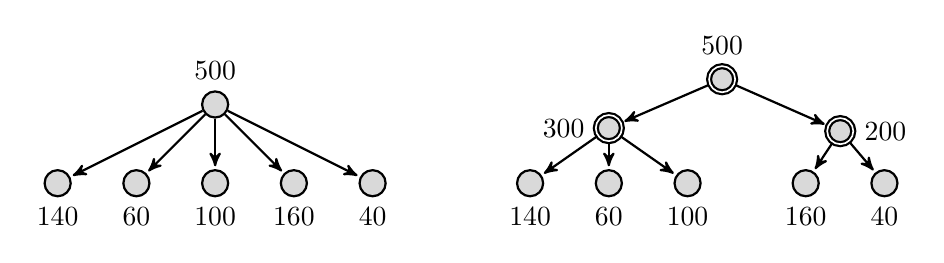
\begin{tikzpicture}[->,>=stealth',shorten >=1pt,auto,node distance=1.cm,
  thick,main node/.style={circle,fill=black!15,draw,font=\sffamily}]

  \node[main node, label=north:500] (1) {};
  \node[main node, label=south:100] (4) [below of=1] {};  
  \node[main node, label=south:60] (3) [left of=4] {};    
  \node[main node, label=south:140] (2) [left of=3] {};  
  \node[main node, label=south:160] (5) [right of=4] {};  
  \node[main node, label=south:40] (6) [right of=5] {}; 

 \node[main node, label=south:140] (7) [right of=6, xshift=1cm] {}; 
 \node[main node, label=south:60] (8) [right of=7] {}; 
 \node[main node, label=south:100] (9) [right of=8] {}; 
 \node[main node, label=south:160] (10) [right of=9, xshift=.5cm] {}; 
 \node[main node, label=south:40] (11) [right of=10] {}; 
  
 \node[main node, yshift=-0.3cm, double,label=west:300] (12) [above of=8] {};
 \node[main node, xshift=.4cm, yshift=-0.3cm, double,label=east:200] (13) [above left = of 11] {};
 \node[main node, xshift=-1.5cm, yshift=-0.7cm, double,label=north:500] (14) [above = of 13] {};
 
  \path[every node/.style={font=\sffamily\tiny}]
    (1) edge node [right] {} (2)
   	    edge node [right] {} (3) 
   	    edge node [right] {} (4)
   	    edge node [right] {} (5)
   	    edge node [right] {} (6)      
    (14) edge node [right] {} (12)
   	     edge node [right] {} (13) 
   	(12) edge node [right] {} (7)
   	     edge node [right] {} (8)
   	     edge node [right] {} (9) 
   	(13) edge node [right] {} (10)
   	     edge node [right] {} (11)      ;
\end{tikzpicture}
\caption{Resource allocation problems can be solved using a hierarchical decomposition structure. Inner nodes representing intermediaries are
marked by double circles.}
\label{fig:hierarchical-decomposition}
\end{figure*}

We present the scheduling problem for some inner node---called intermediary $\AnAvpp$---since the problem is solved top-down, as shown in 
\fref{fig:hierarchical-decomposition}.
Each intermediary in turn redistributes its assigned fraction of the overall demand $\AssResidualLoad{t}{\AnAvpp}$ to 
its subordinate agents $\Subsystem$ until all leaf agents, i.e., physical power plants, are assigned schedules. Note
that the root node $\TlAvpp$ is assigned the actual total demand of the environment, i.e., $\AssResidualLoad{t}{\TlAvpp} = \DemandSym[t]$.
%
\begin{eqnarray}
\label{eq:csop-scheduling-hierarchy} \textstyle
		& \underset{\AgentPower{t}{\AnAgent}}{\operatorname{minimize}} & 
		\alpha_{\ViolationObjective} \cdot \ViolationObjective + \alpha_{\CostsObjective} \cdot \CostsObjective \\
		& \operatorname{subject\ to} & \forall a \in \Subsystem, \forall t \in \Horizon : \exists [x , y] \in \ListProduction{t}\AnAgent : x \leq \AgentPower{t}{\AnAgent} \leq y\text{,} \nonumber \\
		& & \ChangeSpeedMin\AnAgent \left(\AgentPower{t-1}\AnAgent\right) \leq \AgentPower{t}{\AnAgent} \leq \ChangeSpeedMax\AnAgent\left(\AgentPower{t-1}\AnAgent\right) \nonumber\\
		& & \textstyle \text{with } \ViolationObjective = \sum_{t \in \Horizon} \left|\Production_\Subsystem[t] - \AssResidualLoad{t}{\AnAvpp} \right| \text{, } \nonumber \\
		& & \textstyle \text{and } 
		\CostsObjective = \sum_{a \in \Subsystem,\ t \in \Horizon} \CostFunction\AnAgent{\AgentPower{t}{\AnAgent}} \nonumber
\end{eqnarray}
%
We propose to solve this problem using two approaches based on self-organization:
\begin{itemize}
\item A so-called ``regio-central'' approach: agents transfer models to their local supervisor who, at meso-level,
centrally optimizes the allocation~\cite{Schiendorfer2014, SchiendorferSyn2014}
\item An auction-based decentralized approach~\cite{Anders-TAAS-2015}
\end{itemize}

In both cases, obtaining a good abstraction of an intermediary's behavior as a compact
representation of the underlying set of subordinate agents is desirable.

\begin{figure*}
        \centering
        \begin{subfigure}[b]{0.4\textwidth}
        \centering
                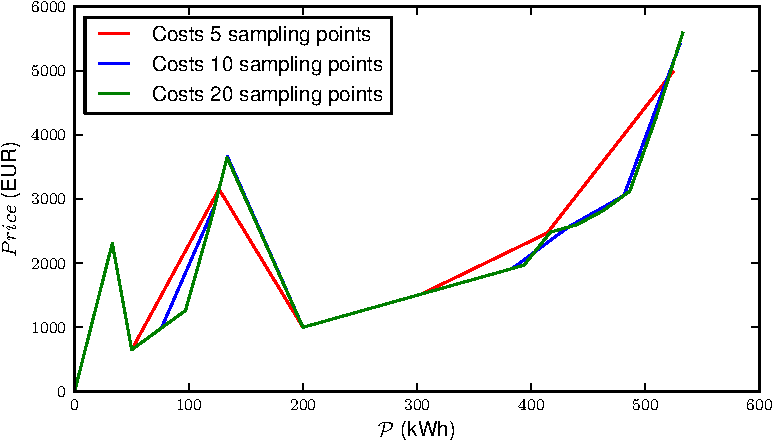
\includegraphics[width=\textwidth]{img/costs}
                \caption{Accuracy affected by the number of sampling points selected.}
                \label{fig:sampling}
        \end{subfigure}%
        ~ \qquad%add desired spacing between images, e. g. ~, \quad, \qquad, \hfill etc.
          %(or a blank line to force the subfigure onto a new line)
        \begin{subfigure}[b]{0.4\textwidth}
        \centering
                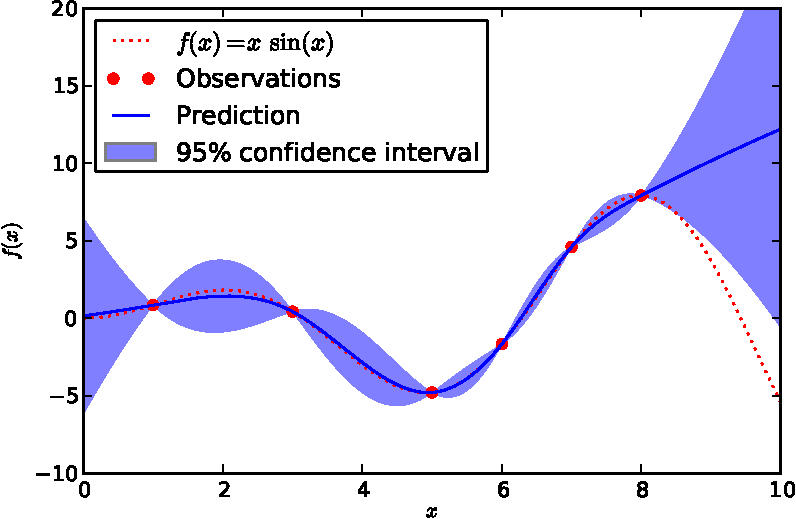
\includegraphics[width=\textwidth]{img/gaussProc}
                \caption{A probabilistic regression model allows to quantify uncertainty at given points in the domain of a learned function.}
                \label{fig:mouse}
        \end{subfigure}
\end{figure*}

%\begin{figure*}
%		\centering
%		 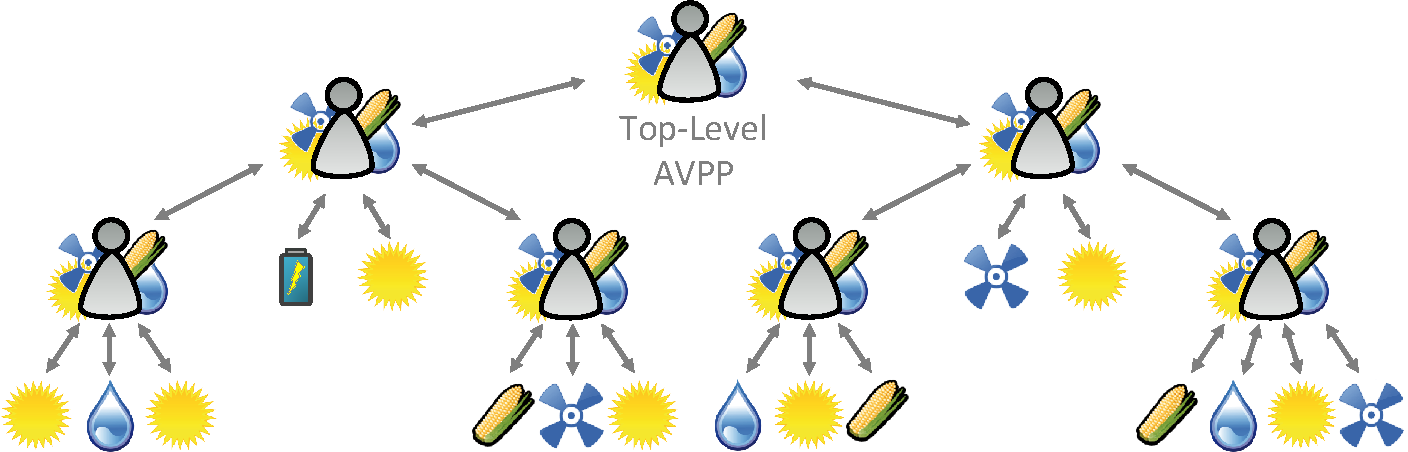
\includegraphics[width=0.55\textwidth]{img/avpp-hierarchical-system-structure.pdf}
%			\caption{Hierarchical system structure of a future autonomous power management system: Prosumers are structured into systems of systems represented by AVPPs acting as intermediaries, thereby decreasing the complexity of control and scheduling. AVPPs can be part of other AVPPs.}
%			%and participate in the power market.}
%		\label{fig:avpp-hierarchical-system-structure}
%\end{figure*}


\section{Issues with Model Abstraction}
However, if
the selected input-output pairs are selected in a weakly informative way, the resulting abstracted
optimization problem introduces severe errors in quality as well as bad runtime performance.

\section{Improving Sampling Point Selection}

\section{Evaluation}
We investigate the effects of selecting a particular set of 
sampling points for one group that could have emerged as part
of a self-organization process.


%\section*{Acknowledgment}
%This research is partly sponsored by the research unit \emph{OC-Trust} (FOR 1085) of the German Research Foundation.

\bibliographystyle{IEEEtran}
\bibliography{saos}

\end{document}
